We will consider two optimality criteria. The first one chooses the states that are individually most likely and maximizes the 
expected number of correct individual states. The second criterion estimates the most likely state sequence, or 
\textit{trellis path}. The algorithm used to implement these criteria is the \textbf{Viterbi} algorithm. %\ref

\section{Noisy Channel Model}

\textbf{FIXME}: Real word spelling error detection is a much more difficult task, since any word in the input text could be 
an error. So we don’t...\\
\textbf{FIXME}{Aggiungere immagine }


We will consider two optimality criteria. The first one chooses the states that are individually most likely and maximizes the 
expected number of correct individual states. The second criterion estimates the most likely state sequence, or 
\textit{trellis path}. The algorithm used to implement these criteria is the \textbf{Viterbi} algorithm. %\ref

\section{Noisy Channel Model}
\textbf{Non-word errors} are detected by looking for any word not found in a dictionary. To correct them we first 
generate \textbf{candidates}, according to a distance given as a parameter to the model (\texttt{edit\_distance}), 
that are 
real words with a similar letter sequence to the error. 

The intuition of the noisy channel model is to treat the misspelled word as if a correctly spelled word had 
been “distorted” by being passed through a noisy communication channel. 
This channel introduces “noise” in the form of substitutions or other changes to the letters, making it hard to 
recognise 
the “true” word. \\

We see an observation $x$ (a misspelled word) and we want to find the word $w$ that generated this misspelled 
word 
(the intended word).
Out of all possible words in the vocabulary $V$ we want to find the word $\hat{w}$ such that $P(\hat{w}|x)$ is 
highest 
among all the candidates $w$
\begin{equation}\label{eq:4.1}
	\hat{w} = \arg\max_{w \in V} P(w|x) \mbox{.}
\end{equation}

This noisy channel model is, therefore, a kind of Bayesian inference, in which it is possible to transform the 
equation 
\ref{eq:4.1} into a set of other probabilities
\begin{equation}\label{eq:4.2}
\hat{w} = \arg\max_{w \in V} \frac{P(x|w)P(w)}{P(x)} \mbox{.}
\end{equation}

Since $P(x)$ doesn’t change for each word because we are always asking about the most likely word for the same 
observed error $x$, we can conveniently simplify the equation \ref{eq:4.2} by dropping the denominator
\begin{equation}\label{eq:4.3}
\hat{w} = \arg\max_{w \in V} {P(x|w)P(w)} \mbox{.}
\end{equation}

\textbf{FIXME}: We apply the noisy channel approach to correcting non-word spelling errors by taking any word not 
in our 
spell dictionary, for example \textsl{adventhre}, generating a list of candidate words like \textsl{adventure}, 
\textsl{adventurer}, \textsl{adventured}, ranking them according to \ref{eq:4.3}, and picking the highest-ranked 
one, 
\textsl{adventure}. \textbf{FIXME}: We choose the most likely candidate, the one with the highest probability.

The two components of the equation are, respectively, $P(x|w)$ the \textbf{channel model} and $P(w)$ the prior 
probability of a hidden word (a candidate).
The prior probability of each correction is the language model probability of the word $w$ in context, which is 
computed using a \textbf{FIXME} \textit{unigram} language model. 
The likelihood is estimated just using the number of times that the a letter $i$ was substituted for the letter $j$ in 
the large corpus of errors \textbf{FIXME} QUALE=? 
To compute the probability for each edit we used a confusion matrix that contains counts of errors. \textbf{FIXME} 
How? 



Each candidate is scored by $P(\mbox{candidate})P(\mbox{typo}|\mbox{candidate})$ and then normalised by the 
sum of the scores for all proposed candidates.

\textbf{FIXME}:  (How is estimated the prior? How are computed the conditional probabilities?)

\begin{figure}[H]
	\centering
	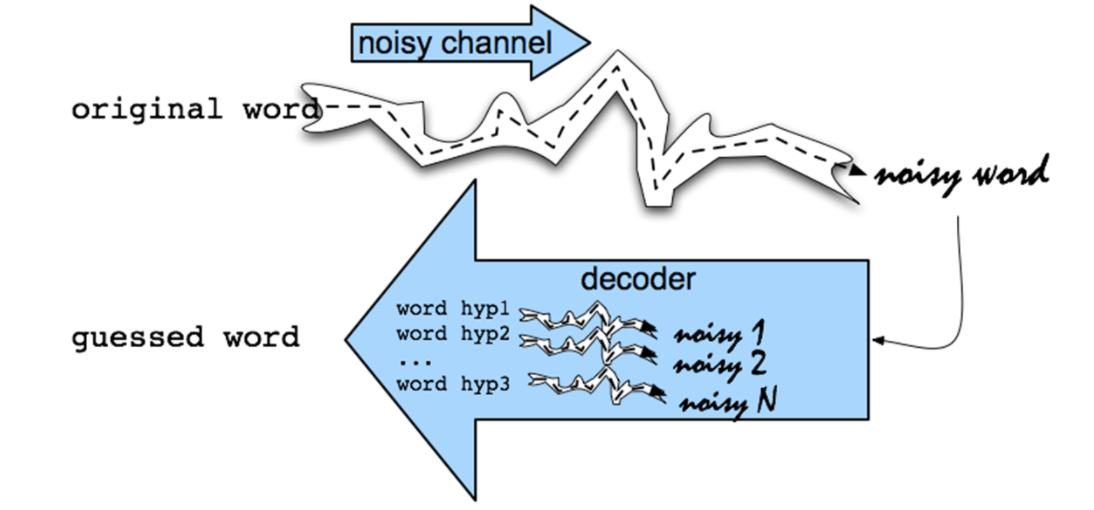
\includegraphics[width=10cm]{NoisyChannel.png}
	\caption{Noisy channel}
	\label{fig:noisychannel}
\end{figure}

\textbf{FIXME}: When for a input typo we do not have any candidate ?? 

\textbf{FIXME}: Real word spelling error detection is a much more difficult task, since any word in the input text 
could be 
an error. So we don’t...\\


To find this list of candidates we uses a minimum edit distance algorithm in the extended version with 
transposition called \textbf{Damerau-Levenshtein} edit distance \ref{}.	\\

The following type of errors were considered in our model:
\begin{itemize}
	\item \textsc{digits deletions}
	\item \textsc{digits insertions}
	\item \textsc{substitutions of digits}: this is the probability to type a character $i$ when the character $j$ was 
	intended ($P(i|j)$). This probability was determined experimentally. \textbf{FIXME}: how? from where?
	\item \textsc{transpositions of adjacent digits}: two letters are swapped.
\end{itemize}

\section{Most Likely State Sequence}

The Viterbi algorithm calculates the most probable sequence of hidden states, the words intended.

The initial probability of being in a state $i$, $\pi_i$, in our case the probability of intend a word $i$, and the 
transition probabilities $A_{ij}$, or the transition from the word $i$ to the next word $j$, are given. Since we have 
observed the output $y_1, y_2, \dots , y_t$, that is the sentence written with typos, it is possible to computed the most 
likely state sequence $x_1, x_2, \dots , x_t$, the sentence intended, starting from the following expression:

\begin{equation}
	\begin{aligned}
		V_{1,t+1} &= P(x_1, \dots, x_t, x_{t+1}, y_1, \dots, y_t,  y_{t+1}) = \\
						&= \arg\max_{x_{1:t}} p(x_1, \dots, x_t | y_1, \dots, y_t) = \\
						& =  \alpha \cdot p(y_{t+1}|x_{t+1})\cdot\max_{x_t} \Big( p(x_{t+1}|x_t) \max p(x_1, \dots, x_{t}|y_1, 
						\dots, y_t)\Big)
	\end{aligned}
\end{equation}

%FIXME
The initial state probabilities $\pi$ are actually the word frequencies (? We don’t estimate it in a proper way), the state 
transition probabilities are given by the probability of a word given its predecessor, \textbf{FIXME}: {come vengono prese} 
and the emission probabilities are the probabilities to type word $i$ when word $j$ was intended.

In our implementation, we construct the \textit{trellis} choosing the \textbf{FIXME}: {locally/globally} best state. As we can 
see in the 
picture below, we display an example of the trellis drawing only the best predecessor of each state.

\begin{figure}[H]
	\centering
	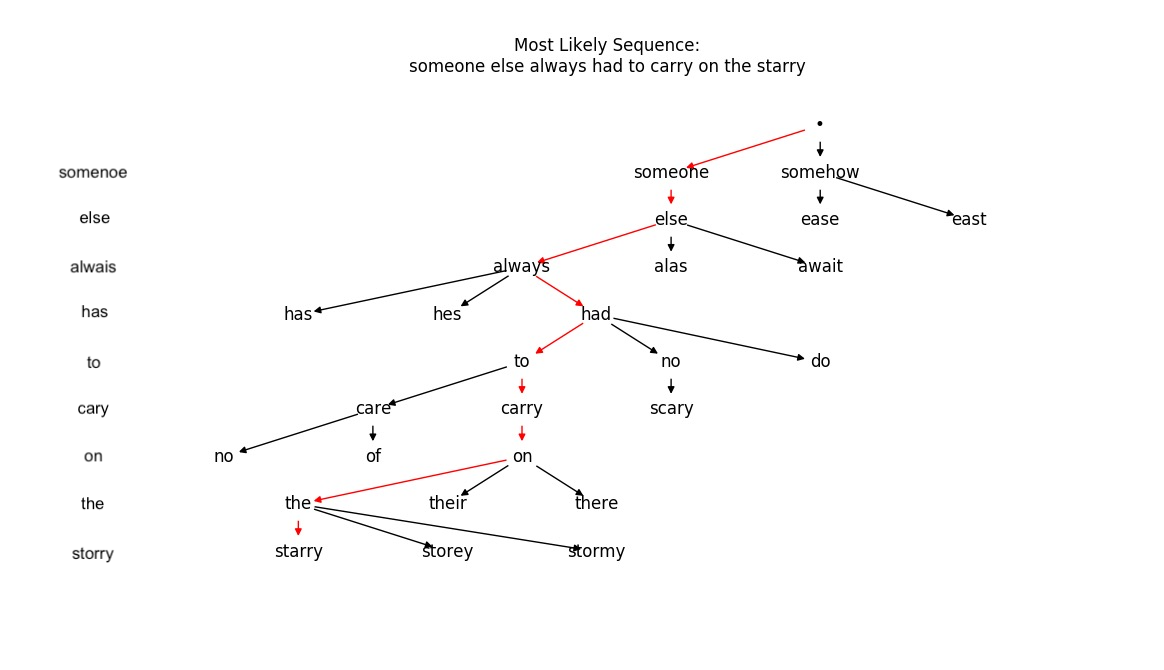
\includegraphics[width=10cm]{TrellisExample.png}
	\caption{Trellis example}
	\label{fig:trellis}
\end{figure}

In this example, we observed the sentence \textsl{my practice iu never iery absorcing} and our algorithm return the most 
likely state sequence \textsl{may practice is never very absorbing}. In this case, the algorithm partially fails, because the 
intended sentence was \textsl{my practice is never very absorbing}.
\\
\textbf{FIXME}: (pi la probabilità iniziale del prima stato non lo abbiamo, non lo facciamo perchè dal nostro dataset non 
abbiamo sempre la prima parola…)

We decide to implement the \textbf{Viterbi} based algorithm instead the Forward-Backward algorithm relying on the 
experiments carried out in the literature.
The HMM-Based Error Correction Mechanism for Five-Key Chording Keyboards article \cite{tarniceriu2015hmm} explains 
that the Forward-Backward algorithm estimates the most likely state for each observation, but the resulting state 
sequence may not be a valid succession of words in natural language (or a very unlikely word sequence) and produce 
inferior results.


\section{Hidden Markov Model}


\textbf{FIXME}: Hmm approach
\textbf{FIXME}: description of hmm

\textbf{FIXME}: our application ...